%
% copied from: https://tikz.net/spherical_volume/
% date: 2023, June 26
%
% adjusted by Alexander Smolka
%
\documentclass[crop,tikz]{standalone}
\usepackage{tikz}
	%\usetikzlibrary{shapes}
	%\usetikzlibrary{automata}
	%\usetikzlibrary{arrows}
	%\usetikzlibrary{backgrounds}
	\usetikzlibrary{calc}
	\usetikzlibrary{positioning}
	\usetikzlibrary{shadings}
	%\usetikzlibrary{patterns}
	%\usetikzlibrary{decorations.pathmorphing}
	%\usetikzlibrary{decorations.pathreplacing}
\usepackage{tikz-3dplot}

\usepackage[scaled]{helvet}
\renewcommand{\familydefault}{\sfdefault}

\input{../../../../../resources/latex/_symbols.qmd}
\begin{document}

\pgfdeclareradialshading[tikz@ball]{ball}{\pgfqpoint{-15bp}{0bp}}{%
 color(0bp)=(tikz@ball!10!white);
 color(9bp)=(tikz@ball!50!white);
 color(18bp)=(tikz@ball!90!black);
 color(25bp)=(tikz@ball!70!black);
 color(50bp)=(black)}

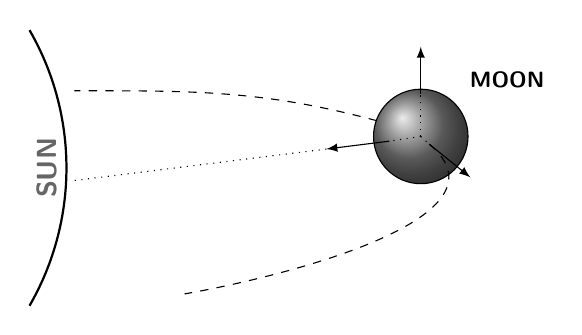
\begin{tikzpicture}[scale=2]
    
    % SUN
    \draw[thick] ($(0,-0.2) + (-30:1.75)$) arc (-30:30:1.75) node[midway, left, rotate=90, anchor=south, fill opacity=0.6] {\textbf{SUN}};

    % MOON
    % \draw[left color=white, right color=black, fill opacity=0.6] (4,0) circle (0.3) node[above right = 0.5 and 0.5] {\footnotesize\textbf{MOON}};
    \draw[ball color=gray] (4,0) circle (0.3) node[above right = 0.5 and 0.5] {\footnotesize\textbf{MOON}};

    \draw[dashed] (4.055,-0.05) to[out=320, in=10] (2.5,-1);
    \draw[dashed] (3.72,0.1) to[out=165, in=0] (1.8,0.29);

    % COORDINATE SYSTEM
    \draw[dotted, thin] (4,0) -- (3.8,-0.03);
    \draw[-latex] (3.8,-0.03) -- +(-0.4,-0.05) node [at end, above left] {$\cartesianCoordinateX$};
    \draw[dotted, thin] (3.4, -0.08) -- +(-1.6, -0.2);

    
    % \draw[dotted, thin] (4,0) -- (3.725,0);
    % \draw[-latex] (3.725,0) -- +(-0.4,0) node [at end, left] {$\cartesianCoordinateX$};

    \draw[dotted, thin] (4,0) -- (4.055, -0.05);
    \draw[-latex] (4.055,-0.05) -- +(0.26,-0.21) node [at end, right] {$\cartesianCoordinateY$};
    \draw[dotted, thin] (4,0) -- (4,0.27);
    \draw[-latex] (4,0.27) -- +(0,0.3) node [at end, above] {$\cartesianCoordinateZ$};

\end{tikzpicture}

\end{document}